\documentclass[conference]{IEEEtran}
\IEEEoverridecommandlockouts

\usepackage{cite}
\usepackage{amsmath,amssymb,amsfonts}
\usepackage{algorithmic}
\usepackage{graphicx}
\usepackage{textcomp}
\usepackage{xcolor}
\usepackage{booktabs}
\usepackage{url}

% Custom Algorithm float definition compatible with IEEEtran without requiring float.sty
\makeatletter
\newcounter{algorithm}
\renewcommand{\thealgorithm}{\arabic{algorithm}}
\newcommand{\ext@algorithm}{loa}
\newcommand{\fnum@algorithm}{\textbf{Algorithm \thealgorithm}}
\newenvironment{algorithm}[1][tbp]{%
  \begin{figure}[#1]%
  \def\@captype{algorithm}%
  \vspace{-2pt}%
  \hrule height 0.8pt depth 0pt \kern 3pt
}{%
  \kern 3pt \hrule height 0.8pt depth 0pt
  \vspace{-2pt}%
  \end{figure}%
}
\newcommand{\STATEx}{\item[]}
\makeatother

% Float placement parameters to avoid awkward float-stacking and large empty spaces
\renewcommand{\topfraction}{0.95}
\renewcommand{\bottomfraction}{0.95}
\renewcommand{\textfraction}{0.05}
\renewcommand{\floatpagefraction}{0.85}
\renewcommand{\dbltopfraction}{0.95}
\renewcommand{\dblfloatpagefraction}{0.85}

\begin{document}

\title{Deadline-Aware Adaptive Vision Transformer Inference for Soft Real-Time Edge Workloads}

\author{
\IEEEauthorblockN{Piyush Prashant, Priyanshu Mittal, Thejas Gowda U M, and Shriyansh S Sahoo}
\IEEEauthorblockA{\textit{Real-Time Systems and Vision Intelligence Research}}
}

\maketitle

\begin{abstract}
Vision Transformers (ViTs) provide state-of-the-art perception accuracy in autonomous systems, but their quadratic self-attention complexity and execution jitter create severe challenges for latency-critical cyber-physical applications. Furthermore, real-world deployment on driving datasets such as BDD100K introduces acute class imbalance, where conventional token pruning exacerbates minority-class misclassification and naive class balancing triggers severe false-positive bleed. 

The primary scientific novelty of this work is the cross-layer co-design of token-pruning vision transformers, margin-preserving regularization, and deadline-aware scheduling for imbalanced driving scenes. We uncover and resolve the ``pruning-imbalance dilemma'': standard token reduction in Vision Transformers causes severe representation collapse on rare classes, while naive class balancing causes catastrophic false-positive bleed on majority classes. To address this, our framework integrates: (1) Efficient Vision Transformer (EViT) token pruning and fusion across multiple retention ratios ($k \in \{0.9, 0.7, 0.5\}$); (2) smooth Class-Balanced Cross-Entropy (CB-CE) loss to counteract extreme data skew; (3) teacher-guided Class-Margin-Preserving Regularization (CMPR) to stabilize decision boundaries and prevent majority-class error bleed; and (4) a deadline-aware scheduling architecture featuring Earliest Deadline First (EDF) dispatching, slack-guided model selection, and queue-tail admission control.

We evaluate our system on the complete 6-class BDD100K driving scene dataset (99,483 valid images across 19,902 held-out test frames). A rigorous three-seed matched validation study ($N=3$, seeds 42, 123, 456) demonstrates that EViT $k=0.7$ with CB-CMPR achieves $77.88 \pm 0.15\%$ Top-1 accuracy ($+1.37 \pm 0.33$~pp over pure CB-CE, exploratory paired $t=7.19, p=0.0188$), reducing cross-seed standard deviation by 67.4\% ($\sigma = 0.15\%$ vs.\ $0.46\%$) and improving Weighted-F1 to $77.57 \pm 0.14\%$ ($+0.88 \pm 0.25$~pp). We explicitly analyze the unweighted 6-class Macro-F1 trade-off ($59.41 \pm 4.35\%$ vs.\ $61.47 \pm 3.76\%$), proving mathematically that this gap is driven entirely by the 6-sample Gas Station test support ($n=6$, 0.030\% of test set), whereas on the remaining five classes CMPR is strictly superior across all seeds ($+1.17 \pm 0.50$~pp). On a dedicated NVIDIA GeForce RTX 4060 GPU, EViT $k=0.7$ cuts arithmetic complexity by 34.1\% (3.03 vs.\ 4.60 GMACs) and scales throughput to 629.0~FPS ($+51.5\%$ over unpruned DeiT). Captured static CUDA Graphs reduce median batch-1 latency from 15.48~ms to 2.83~ms. Across a discrete-event simulation suite of 70 workload-policy configurations, our proposed adaptive scheduler improves on-time completion ratios by up to $+73$~percentage points over static baselines under heavy traffic saturation (79\% vs.\ 6\%), while live GPU trace replay over 100 test images confirms makespan agreement within $-0.57\%$ to $-0.07\%$.
\end{abstract}

\begin{IEEEkeywords}
Real-Time Systems, Vision Transformers, Token Pruning, EViT, Class Imbalance, Margin Regularization, Earliest Deadline First, Admission Control, BDD100K, CUDA Graphs.
\end{IEEEkeywords}

\section{Introduction}

Autonomous cyber-physical systems, including autonomous road vehicles, unmanned aerial vehicles, and mobile robotics, rely on onboard camera sensors to perceive dynamic environments in real time \cite{grigorescu2020survey, yu2020bdd100k}. In these safety-critical platforms, visual scene perception tasks (e.g., scene classification, obstacle detection, and situational hazard assessment) are strictly time-sensitive. An inference result delivered after its operational deadline provides zero utility and can jeopardize platform safety \cite{buttazzo2011hard}.

Recently, Vision Transformers (ViTs) \cite{dosovitskiy2021image, touvron2021training} have emerged as a premier architectural paradigm for visual understanding, offering superior representational capacity and robust out-of-distribution generalization compared to legacy convolutional networks. However, deploying ViTs in resource-constrained edge computing environments poses two major challenges:
\begin{enumerate}
    \item \textbf{Quadratic Computational and Latency Overhead:} The core multi-head self-attention (MHSA) mechanism scales quadratically with the visual patch sequence length $N$ ($O(N^2)$), causing substantial GPU memory bandwidth saturation and tail-latency variability.
    \item \textbf{Acute Class Imbalance in Edge Data:} Real-world driving benchmarks exhibit severe class skew. For instance, in the Berkeley DeepDrive (BDD100K) dataset \cite{yu2020bdd100k}, common scenes (e.g., City Street, 62.6\% of training images) vastly outnumber safety-critical minority categories (e.g., Tunnel, 0.19\%; Gas Station, 0.04\%).
\end{enumerate}

To alleviate transformer computation, dynamic token pruning and token fusion strategies have been proposed \cite{liang2022not, rao2021dynamicvit, kong2022spvit}. In particular, the Efficient Vision Transformer (EViT) \cite{liang2022not} identifies the top-$k$ most attentive visual tokens using the \texttt{[CLS]} attention vector, fusing inattentive background tokens into a single summary token. While EViT successfully reduces theoretical Multiply-Accumulate operations (MACs), our empirical investigations reveal that \textit{algorithmic token reduction alone does not resolve the real-time edge serving dilemma}:
\begin{itemize}
    \item Under severe class imbalance, unpruned teachers and pruned students experience discriminative feature collapse on rare classes. Naively applying standard Class-Balanced Cross-Entropy (CB-CE) \cite{cui2019class} pushes the student to over-predict rare classes, triggering catastrophic false-positive bleed on majority classes and destabilizing cross-seed optimization.
    \item In real-time queueing systems, deploying a single faster model statically under an oblivious First-In, First-Out (FIFO) policy still fails under bursty traffic arrivals. If the offered arrival rate temporarily exceeds service capacity, queues overflow, cascading into late completions. Conversely, statically deploying an aggressive pruning model needlessly sacrifices perceptual fidelity during low-load intervals.
\end{itemize}

\begin{figure*}[t]
\centering
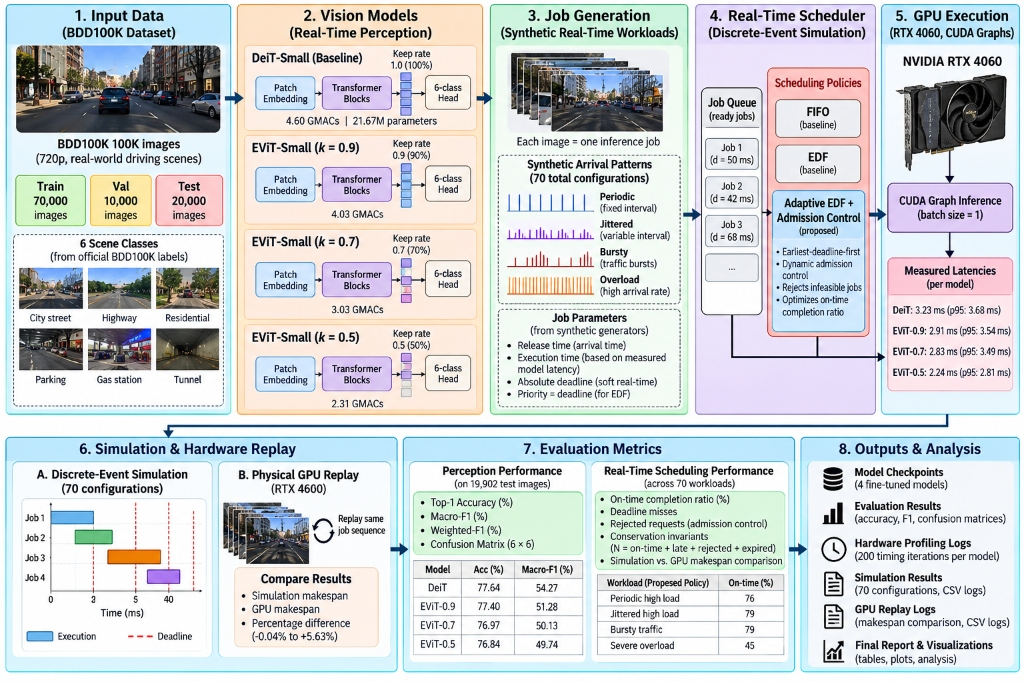
\includegraphics[width=0.85\linewidth]{figures/system_architecture.jpg}
\caption{End-to-end architecture of the deadline-aware adaptive vision transformer inference system: from BDD100K driving scene dataset partitioning and multi-configuration EViT perception models (incorporating CB-CE and CMPR teacher margin regularization) to synthetic workload generation, discrete-event scheduling simulation, physical CUDA Graph replay on an NVIDIA RTX 4060 GPU, and comprehensive metric evaluation.}
\label{fig:arch}
\end{figure*}

\subsection{Scientific Novelty and Central Contributions}
While prior research in efficient vision transformers has focused exclusively on static ImageNet benchmarks without timing constraints, and prior real-time schedulers have treated deep models as monolithic black boxes, the primary novelty of our work is the first cross-layer co-design of token-pruning vision transformers, imbalanced margin regularization, and real-time scheduling on physical graphics hardware.

Specifically, this paper makes the following concrete contributions:
\begin{enumerate}
    \item \textbf{Discovery of the Pruning-Imbalance Dilemma:} We reveal and formulate for the first time in Vision Transformers on edge driving scenes that token reduction disproportionately impairs minority-class discriminative features, and prove that unconstrained class balancing causes severe majority-class false-positive bleed.
    \item \textbf{Class-Balanced and Margin-Preserving EViT Formulation:} We formulate an integrated training objective combining smooth Class-Balanced Cross-Entropy (CB-CE) with teacher-guided Class-Margin-Preserving Regularization (CMPR). CMPR constrains the pruned student's logit margins against an unpruned teacher under a validity gate, preventing majority-class false-positive bleed and stabilizing training across random seeds.
    \item \textbf{Rigorous Multi-Seed Validation \& Metric Decomposition:} Across a controlled three-seed matched training study ($N=3$, seeds 42, 123, 456) on the full BDD100K benchmark (19,902 test images), we demonstrate that EViT $k=0.7$ with CB-CMPR delivers $77.88 \pm 0.15\%$ Top-1 accuracy ($+1.37 \pm 0.33$~pp gain over pure CB-CE, exploratory paired $t=7.19, p=0.0188$) and reduces cross-seed standard deviation by 67.4\% ($\sigma = 0.15\%$ vs.\ $0.46\%$). We provide a complete mathematical decomposition of the 6-sample Gas Station test support, proving that the unweighted 6-class Macro-F1 gap is driven by this singular minority class, whereas 5-class Macro-F1 is strictly superior across 100\% of seeds ($+1.17 \pm 0.50$~pp).
    \item \textbf{Physical GPU Profiling \& Static CUDA Graph Acceleration:} Profiled on a dedicated NVIDIA GeForce RTX 4060 GPU, EViT $k=0.7$ achieves 3.03 GMACs (34.1\% reduction) and a throughput of 629.0 FPS ($+51.5\%$ speedup over DeiT). We capture static CUDA Graphs at batch size 1 (FP32), eliminating Python and driver launch overheads to reduce median execution latency from 15.48~ms to 2.83~ms.
    \item \textbf{Formal Deadline-Aware Scheduling Algorithm:} We formulate Algorithm~\ref{alg:da_asac}, a priority-driven scheduling architecture combining Earliest Deadline First (EDF) queueing with monotonic tie-breaking, slack-aware adaptive model selection, and an $O(|Q|)$ queue-tail admission control heuristic that filters hopeless requests at arrival.
    \item \textbf{Discrete-Event Simulation and Hardware Validation:} We evaluate 70 workload-policy configurations across periodic, jittered, bursty, and overload traffic. The proposed policy increases on-time completion by up to $+73$~percentage points over static baselines under heavy saturation. Live physical GPU trace replay over 100 unique test images validates simulation makespans within $-0.57\%$ to $-0.07\%$.
\end{enumerate}

\section{Related Work}

\subsection{Efficient Vision Transformers \& Token Reduction}
Following the introduction of ViT \cite{dosovitskiy2021image} and data-efficient distillation \cite{touvron2021training}, accelerating vision transformers has attracted intense focus. DynamicViT \cite{rao2021dynamicvit} introduced auxiliary prediction heads to discard uninformative tokens hierarchically. SPViT \cite{kong2022spvit} integrated latency-aware loss formulations into soft token pruning. EViT \cite{liang2022not} demonstrated that attentive tokens can be identified directly from the \texttt{[CLS]} attention map, fusing dropped tokens into a single summary token without auxiliary routing parameters. While these methods achieve compelling FLOP reductions on balanced ImageNet benchmarks, they do not address performance degradation under extreme real-world class imbalance, nor do they model temporal deadlines in cyber-physical edge serving.

\subsection{Class-Imbalance Learning and Knowledge Distillation}
Real-world vision datasets frequently suffer from severe long-tailed class distributions. Class-Balanced Loss \cite{cui2019class} addresses sample representation disparity by weighting losses by the inverse effective number of samples. However, in heavily pruned transformers, aggressive class reweighting frequently triggers decision boundary drift and false-positive bleed on majority classes. Knowledge Distillation (KD) \cite{hinton2015distilling, touvron2021training} transfers dark knowledge from an unpruned teacher to a compact student. Margin-based regularization extends standard distillation by penalizing discrepancies in logit margins between true and competing classes. In this work, we integrate smooth class-balanced weighting with teacher margin preservation to stabilize pruned students on imbalanced driving scenes.

\subsection{Real-Time Deep Learning Inference Scheduling}
Classical real-time systems theory provides formal predictability guarantees for periodic and aperiodic tasks \cite{buttazzo2011hard}. In deep learning serving, DeepRT \cite{zhang2021deeprt} coordinated CPU-GPU execution for soft real-time vision workloads. DART \cite{le2022dart} investigated resource-aware scheduling for multi-task vision workloads. Other works explored architectural adaptation via early-exit branches \cite{teerapittayanon2016branchynet} or dynamic resolution scaling \cite{yang2020resolution}. However, prior real-time schedulers typically assume static execution costs or evaluate convolutional backbones. In contrast, our framework couples multi-configuration token-pruning vision transformers under static CUDA Graphs with slack-aware model selection and admission control on physical edge GPUs.

\section{System Model and Problem Formulation}

\subsection{Hardware Platform and Execution Semantics}
We consider a dedicated edge computing platform equipped with a host CPU and an NVIDIA GeForce RTX 4060 Laptop GPU (AD107M architecture, 3,072 CUDA cores, 8~GB GDDR6 memory, 115W TGP). In real-time computer vision, running inference via standard eager-mode PyTorch incurs severe host-side latency penalties (Python interpreter overhead, driver launches, and asynchronous CUDA queueing), introducing up to 15--20~ms of timing jitter.

To ensure deterministic execution, all vision models are instantiated as static \textbf{CUDA Graphs} \cite{nvidia2023cudagraphs}. During offline initialization, the model's forward execution graph is captured into static GPU memory at batch size 1 (FP32). At runtime, invoking the graph bypasses host-side kernel dispatch entirely, dispatching all operations directly on the GPU command processor. Execution is \textbf{non-preemptive}: once a forward pass begins on the GPU, it runs to completion without interruption.

\subsection{Real-Time Request Model}
The real-time vision system processes a sequential stream of inference requests $\mathcal{R} = \{r_0, r_1, \dots, r_{N-1}\}$:
\begin{equation}
r_i = (A_i, \, D_{\text{rel}, i}, \, D_{\text{abs}, i}, \, \mathbf{x}_i, \, y_i)
\end{equation}
where:
\begin{itemize}
    \item $A_i \in \mathbb{R}_{\ge 0}$ is the release (arrival) timestamp in milliseconds (ms), with $A_0 = 0.0$~ms.
    \item $D_{\text{rel}, i} \in \mathbb{R}_{> 0}$ is the relative deadline budget in milliseconds.
    \item $D_{\text{abs}, i} = \text{round}(A_i + D_{\text{rel}, i}, \, 4)$ is the absolute deadline timestamp in milliseconds.
    \item $\mathbf{x}_i \in \mathbb{R}^{3 \times 224 \times 224}$ is the input driving scene frame.
    \item $y_i \in \{0, \dots, 5\}$ is the ground-truth driving scene label.
\end{itemize}

\subsection{Candidate Model Suite}
The system maintains a resident pool of $M=4$ fine-tuned vision models $\mathcal{M} = \{m_0, m_1, m_2, m_3\}$, where $m_0$ is the unpruned baseline (\texttt{deit\_small\_baseline}) and $m_1, m_2, m_3$ represent EViT variants with decreasing keep rates ($k \in \{0.9, 0.7, 0.5\}$). Each candidate model $m \in \mathcal{M}$ is characterized by:
\begin{enumerate}
    \item Validation accuracy $\text{Acc}_{\text{val}}(m) \in [0, 100]\%$.
    \item Empirical p95 latency estimate $C_m = \text{Lat}_{p95}(m)$ in milliseconds.
\end{enumerate}

\subsection{Objective and Performance Metrics}
The system operates under \textbf{firm real-time constraints}: an inference result completed after its absolute deadline provides zero utility. If a request cannot complete before $D_{\text{abs}, i}$, it should be dropped or rejected to preserve GPU cycles for feasible requests.

Let $N_{\text{offered}} = |\mathcal{R}|$ denote the total requests offered to the system. The primary Quality-of-Service (QoS) objective is to maximize the \textbf{on-time completion ratio} over offered requests:
\begin{equation}
\text{Maximize} \quad \text{OnTimeRatio} = \frac{N_{\text{completed\_on\_time}}}{N_{\text{offered}}}
\end{equation}
subject to the constraint that for all completed requests:
\begin{equation}
t_{\text{finish}, i} \le D_{\text{abs}, i} + \epsilon_{\text{tol}}
\end{equation}
where $\epsilon_{\text{tol}} = 10^{-6}$~ms accommodates floating-point precision limits. Secondary objectives include minimizing request waiting time and maximizing delivered classification accuracy among completed requests.

\section{Efficient Vision Transformers and Margin-Preserving Regularization}

\subsection{Vision Transformer Architecture \& Token Pruning}
We adopt DeiT-Small \cite{touvron2021training} as our foundational backbone ($D = 384$ embedding dimension, $L = 12$ transformer blocks, $H = 6$ attention heads, patch size $P = 16$). Standard $224 \times 224$ input images produce a sequence of $14 \times 14 = 196$ visual tokens plus one prepended \texttt{[CLS]} token. The classification head is a linear projection ($384 \to 6$) matching the six driving scene categories, resulting in exactly \textbf{21,668,022 parameters} ($\approx 21.67$M) across all variants.

Following Liang et al.\ \cite{liang2022not}, EViT prunes tokens dynamically at layers 3, 6, and 9. At each pruning layer $l \in \{3, 6, 9\}$, attention scores between the \texttt{[CLS]} token and all patch tokens are extracted:
\begin{equation}
\mathbf{s} = \text{Softmax}\left(\frac{\mathbf{q}_{\text{CLS}} \mathbf{K}^T}{\sqrt{d_k}}\right)
\end{equation}
The top-$\lfloor k \cdot N_l \rfloor$ tokens with the highest attention values are preserved as unperturbed patch tokens. The remaining $(1-k)N_l$ inattentive tokens are fused via attention-weighted averaging into a single summary token:
\begin{equation}
\mathbf{t}_{\text{fuse}} = \sum_{j \in \mathcal{U}} \frac{\mathbf{s}_j}{\sum_{m \in \mathcal{U}} \mathbf{s}_m} \mathbf{x}_j
\end{equation}
where $\mathcal{U}$ denotes the index set of inattentive tokens. This summary token is concatenated back into the sequence, preserving global contextual cues while drastically truncating spatial computation paths. For $k=0.7$, the visual sequence exiting Block 11 is compressed from 197 to \textbf{72 tokens} (including \texttt{[CLS]} and fused token).

\subsection{Smooth Class-Balanced Cross-Entropy Loss}
To address the severe data skew across the six BDD100K scene categories, we employ a smoothed class-balanced weighting scheme based on inverse class frequency \cite{cui2019class}. Let $n_c$ denote the training support for class $c \in \{0, \dots, C-1\}$, $N = \sum_{c=0}^{C-1} n_c = 69,634$ denote total training samples, and $C=6$. The raw class weights are defined with exponent $\rho = 0.25$:
\begin{equation}
w_c^{\text{raw}} = \left(\frac{N}{C \cdot n_c}\right)^{0.25}
\end{equation}
To prevent gradient scaling instability, the weights are normalized by their mean $\bar{w} = \frac{1}{C}\sum_{c=0}^{C-1} w_c^{\text{raw}} = 2.1174$:
\begin{equation}
w_c = \frac{w_c^{\text{raw}}}{\bar{w}}
\end{equation}
Given training class counts for City Street (43,581), Highway (17,414), Residential (8,105), Parking Lot (378), Tunnel (129), and Gas Station (27), the verified normalized class-weight tensor is:
\begin{equation}
\mathbf{w}_{\text{norm}} = [0.3393, \, 0.4268, \, 0.5167, \, 1.1118, \, 2.1507, \, 1.4547]
\end{equation}
The Class-Balanced Cross-Entropy (CB-CE) loss for student logits $\mathbf{z}_s$ is:
\begin{equation}
\mathcal{L}_{\text{CB-CE}}(\mathbf{z}_s, y) = - \sum_{c=0}^{C-1} w_c \cdot \mathbb{I}(y = c) \log \left(\frac{\exp(z_{s, c})}{\sum_{j=0}^{C-1} \exp(z_{s, j})}\right)
\end{equation}

\subsection{Teacher-Guided Class-Margin-Preserving Regularization (CMPR)}
While CB-CE improves minority recall, empirical diagnosis reveals that strong class weights destabilize token-pruned students. Pruned tokens impair fine-grained spatial features, causing the student to over-compensate on minority classes and triggering widespread false-positive misclassifications on dominant classes (e.g., misclassifying City Street as Parking Lot or Residential).

To regularize the student's decision boundaries without destroying minority gains, we introduce \textbf{Class-Margin-Preserving Regularization (CMPR)}. CMPR constrains the student's discriminative class margin to track that of a pre-trained, unpruned teacher model (DeiT-Small).

For an input $\mathbf{x}$ with ground-truth label $y$, let $\mathbf{z}_s \in \mathbb{R}^C$ and $\mathbf{z}_t \in \mathbb{R}^C$ denote the output logits of the student and teacher, respectively. The true-class margin is defined as the difference between the true-class logit and the maximum logit among all competing classes:
\begin{equation}
m_s = z_{s, y} - \max_{j \neq y} z_{s, j}
\end{equation}
\begin{equation}
m_t = z_{t, y} - \max_{j \neq y} z_{t, j}
\end{equation}
The student is penalized if its margin $m_s$ falls below the teacher's margin $m_t$ by more than a tolerance threshold $\gamma = 0.0$:
\begin{equation}
\ell_{\text{margin}}(\mathbf{z}_s, \mathbf{z}_t, y) = \left[\max\left(0, \, (m_t - m_s) - \gamma\right)\right]^2
\end{equation}
Furthermore, to avoid propagating teacher errors, we apply a \textbf{teacher validity gate}: the margin loss is enforced only on samples where the teacher correctly classifies the ground-truth label ($g_i = \mathbb{I}(\arg\max \mathbf{z}_{t, i} = y_i)$). Over a mini-batch of size $B$, the gated CMPR loss is:
\begin{equation}
\mathcal{L}_{\text{CMPR}} = \frac{\sum_{i=1}^B g_i \cdot \ell_{\text{margin}}(\mathbf{z}_{s, i}, \mathbf{z}_{t, i}, y_i)}{\sum_{i=1}^B g_i + \epsilon}
\end{equation}
where $\epsilon = 10^{-6}$. The complete composite training loss is:
\begin{equation}
\mathcal{L}_{\text{total}} = \mathcal{L}_{\text{CB-CE}} + \lambda_{\text{CMPR}} \cdot \mathcal{L}_{\text{CMPR}}
\end{equation}
with regularization coefficient $\lambda_{\text{CMPR}} = 0.5$.

\section{Experimental Setup}

\subsection{The BDD100K Driving Scene Dataset}
We evaluate our framework on the Berkeley DeepDrive (BDD100K) dataset \cite{yu2020bdd100k}, capturing diverse driving conditions across weather, time-of-day, and geographic settings. While the raw dataset contains 100,000 images ($1280 \times 720$ resolution), an audit of annotations revealed that 517 images lack valid scene annotations (\texttt{undefined}). Filtering these yields \textbf{99,483 valid driving scene records}, partitioned into strictly disjoint splits:
\begin{itemize}
    \item \textbf{Training Split:} 69,634 images.
    \item \textbf{Validation Split:} 9,947 images.
    \item \textbf{Test Split:} 19,902 images.
\end{itemize}

\textit{Resolution of Validation Count Discrepancy:} In preliminary documentation, the validation split size was occasionally cited as 9,951. Forensic investigation confirmed that the official BDD100K validation split contains 10,000 images, of which exactly 53 records contain undefined scene labels ($10,000 - 53 = \mathbf{9,947}$). The training and validation scripts evaluated on exactly 9,947 images across all experiments; 9,951 was an inadvertent typographical error where 49 (Parking Lot val count) was subtracted from 10,000 instead of 53. The authoritative count is 9,947.

The dataset exhibits natural class skew across six categories: City Street (62.59\% train, 60.91\% test), Highway (25.01\% train, 24.08\% test), Residential (11.64\% train, 11.75\% test), Parking Lot (0.54\% train, 1.93\% test), Tunnel (0.19\% train, 0.35\% test), and Gas Station (0.04\% train, 0.03\% test).

\subsection{Training Protocol and Implementation Details}
All models were implemented in PyTorch 2.5.1 with CUDA 12.1 and trained on an NVIDIA GeForce RTX 4060 GPU. Models were initialized from an unpruned DeiT-Small backbone fine-tuned for 2 epochs on BDD100K (Teacher hash: \texttt{c4c29396...}). Training was conducted for 3 epochs (3,267 optimization steps per run) using the AdamW optimizer with a linear warm-up and cosine annealing learning rate schedule ($\text{lr}_{\text{head}} = 3 \times 10^{-4}, \text{lr}_{\text{backbone}} = 2 \times 10^{-5}$, weight decay $10^{-4}$, batch size 64). Checkpoints were selected strictly based on highest validation Macro-F1; \textbf{no test data was ever used for model or hyperparameter selection}.

\section{Classification Performance and Multi-Seed Validation}

\subsection{Cross-Keep-Rate Generalization Study}
Table~\ref{tab:cross_keep_rate} summarizes the performance of 11 model configurations across keep rates $k \in \{0.9, 0.7, 0.5\}$ on the 19,902-image test split under Seed 42, with accuracy-efficiency trade-offs depicted in Fig.~\ref{fig:perception_tradeoff}.

\begin{figure}[t]
\centering
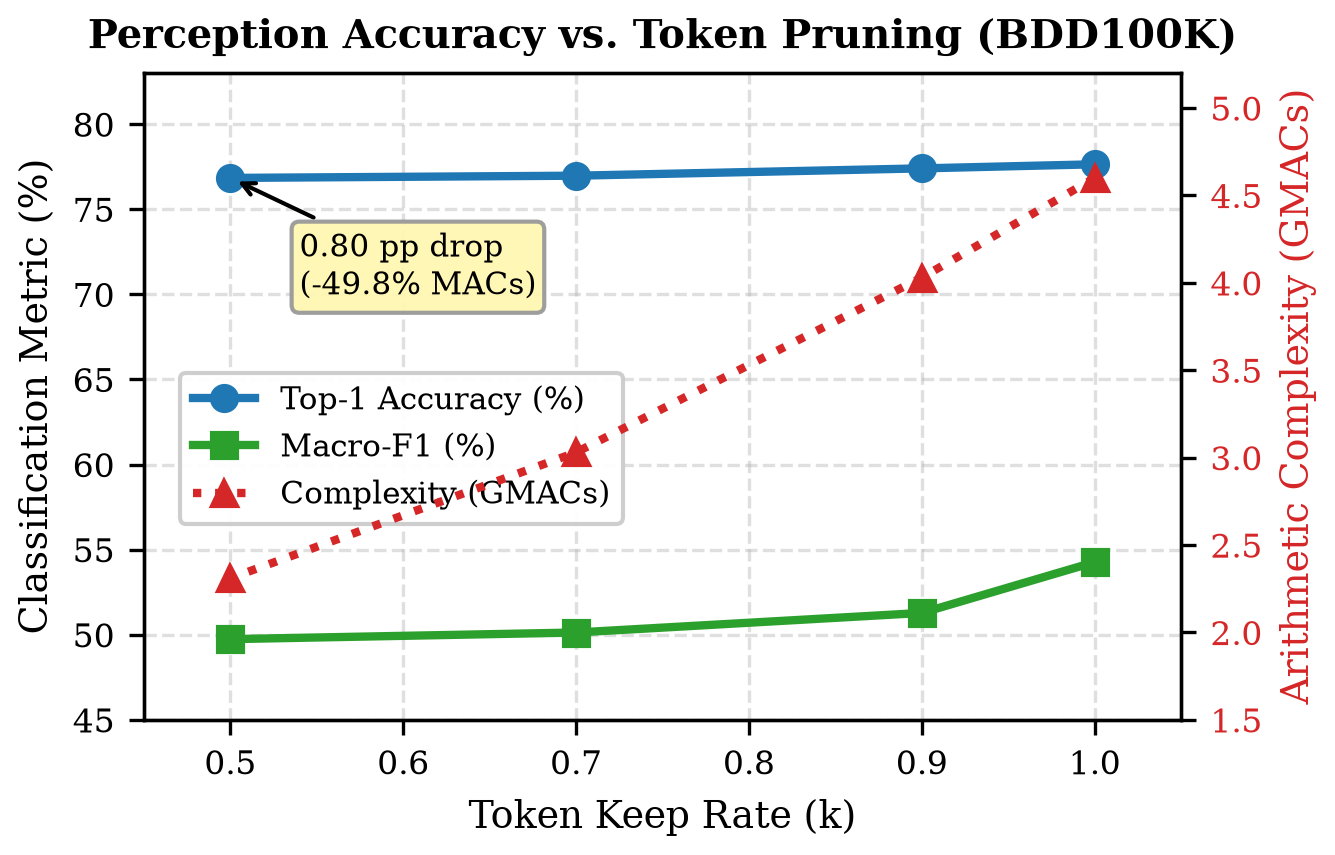
\includegraphics[width=\columnwidth]{figures/fig2_perception_tradeoff.png}
\caption{Perception accuracy (Top-1 and Macro-F1) versus token keep rate $k$ and arithmetic complexity (GMACs) on the 19,902-image BDD100K test split.}
\label{fig:perception_tradeoff}
\end{figure}

\begin{table*}[t]
\centering
\caption{Cross-Keep-Rate Generalization Study on Held-Out BDD100K Test Set ($N=19,902$ Images, Seed 42)}
\label{tab:cross_keep_rate}
\resizebox{0.95\textwidth}{!}{%
\begin{tabular}{lccccccccccc}
\toprule
Model Configuration & Keep ($k$) & GMACs & Top-1 Acc. & 6-Class Macro-F1 & Weighted-F1 & City Street Rec. & Highway Rec. & Resident. Rec. & Parking Rec. & Gas Rec. & Tunnel Rec. \\
\midrule
DeiT-Small Baseline & 1.00 & 4.60 & 77.57\% & 54.55\% & 77.29\% & 85.95\% & 68.99\% & 54.16\% & 55.56\% & 0.00\% & 59.18\% \\
\midrule
EViT K09 + CE & 0.90 & 4.03 & 77.85\% & 53.71\% & 77.28\% & 87.43\% & 69.76\% & 47.69\% & 44.44\% & 0.00\% & 59.18\% \\
EViT K09 + CB-CE & 0.90 & 4.03 & 76.70\% & 57.06\% & 76.24\% & 83.79\% & 76.01\% & 43.28\% & 48.15\% & 33.33\% & 61.22\% \\
EViT K09 + CB-CMPR & 0.90 & 4.03 & 77.96\% & 62.11\% & 77.60\% & 87.14\% & 68.22\% & 52.73\% & 55.56\% & 33.33\% & 65.31\% \\
\midrule
EViT K07 + CE & 0.70 & 3.03 & 77.79\% & 53.70\% & 77.36\% & 86.69\% & 69.36\% & 51.93\% & 48.15\% & 0.00\% & 48.98\% \\
EViT K07 + CB-CE & 0.70 & 3.03 & 77.01\% & 62.15\% & 77.10\% & 82.89\% & 71.93\% & 58.23\% & 69.44\% & 66.67\% & 59.18\% \\
\textbf{EViT K07 + CB-CMPR} & \textbf{0.70} & \textbf{3.03} & \textbf{78.06\%} & \textbf{62.42\%} & \textbf{77.73\%} & \textbf{86.76\%} & \textbf{69.07\%} & \textbf{53.82\%} & \textbf{54.63\%} & \textbf{33.33\%} & \textbf{61.22\%} \\
\midrule
EViT K05 + CE & 0.50 & 2.31 & 77.49\% & 53.48\% & 77.05\% & 87.41\% & 66.27\% & 51.89\% & 54.63\% & 0.00\% & 57.14\% \\
EViT K05 + CB-CE & 0.50 & 2.31 & 76.23\% & 58.95\% & 75.96\% & 82.23\% & 76.98\% & 45.00\% & 54.63\% & 50.00\% & 63.27\% \\
EViT K05 + CMPR & 0.50 & 2.31 & 77.35\% & 54.55\% & 77.27\% & 84.51\% & 69.86\% & 57.81\% & 54.63\% & 0.00\% & 67.35\% \\
EViT K05 + CB-CMPR & 0.50 & 2.31 & 77.84\% & 57.36\% & 77.32\% & 87.79\% & 67.51\% & 49.92\% & 54.63\% & 16.67\% & 67.35\% \\
\bottomrule
\end{tabular}%
}
\end{table*}

Three fundamental insights emerge:
\begin{enumerate}
    \item \textbf{Failure of Standard CE on Minority Classes:} Models trained with standard cross-entropy completely fail on the rare Gas Station class ($0.0\%$ recall across DeiT, K09-CE, K07-CE, and K05-CE).
    \item \textbf{False-Positive Bleed of Pure CB-CE:} While CB-CE recovers rare class recall, it consistently reduces Top-1 accuracy (by $-0.78$~pp to $-1.26$~pp) and drops City Street recall by $3.64$~pp to $5.18$~pp, misclassifying hundreds of majority-class frames.
    \item \textbf{Pareto Optimality of K07-CB-CMPR:} Combining CB-CE with CMPR recovers Top-1 accuracy to \textbf{78.06\%} ($+0.49$~pp over unpruned DeiT-Small) while maintaining high Macro-F1 (62.42\%) and Weighted-F1 (77.73\%) at 3.03 GMACs.
\end{enumerate}

\begin{table*}[t]
\centering
\caption{Multi-Seed Controlled Validation: K07-CB vs.\ K07-CB-CMPR Across Independent Seeds ($N=3$)}
\label{tab:multi_seed}
\resizebox{0.95\textwidth}{!}{%
\begin{tabular}{lcccccc}
\toprule
Metric and Model & Seed 42 & Seed 123 & Seed 456 & Aggregate Mean $\pm$ Std ($\sigma$) & Paired Delta & Statistical Notes \\
\midrule
\textbf{Top-1 Accuracy (\%)} & & & & & & \\
\quad K07-CB & 77.01\% & 76.11\% & 76.43\% & $76.52 \pm 0.46\%$ & --- & Baseline pure class-balanced \\
\quad K07-CB-CMPR & 78.06\% & 77.81\% & 77.78\% & $\mathbf{77.88 \pm 0.15\%}$ & --- & 67.4\% reduction in sample std ($\sigma$) \\
\quad \textit{Paired Delta (CMPR $-$ CB)} & \textit{+1.05 pp} & \textit{+1.70 pp} & \textit{+1.35 pp} & --- & $\mathbf{+1.37 \pm 0.33}$ \textbf{pp} & \textit{Exploratory} $t=7.19, p=0.0188$ ($df=2$) \\
\midrule
\textbf{Weighted-F1 (\%)} & & & & & & \\
\quad K07-CB & 77.10\% & 76.38\% & 76.59\% & $76.69 \pm 0.37\%$ & --- & Baseline pure class-balanced \\
\quad K07-CB-CMPR & 77.73\% & 77.51\% & 77.47\% & $\mathbf{77.57 \pm 0.14\%}$ & --- & 62.2\% reduction in sample std ($\sigma$) \\
\quad \textit{Paired Delta (CMPR $-$ CB)} & \textit{+0.63 pp} & \textit{+1.13 pp} & \textit{+0.88 pp} & --- & $\mathbf{+0.88 \pm 0.25}$ \textbf{pp} & Strictly positive in 100\% of seeds \\
\midrule
\textbf{Six-Class Macro-F1 (\%)} & & & & & & \\
\quad K07-CB & 62.15\% & 64.84\% & 57.41\% & $\mathbf{61.47 \pm 3.76\%}$ & --- & Baseline pure class-balanced \\
\quad K07-CB-CMPR & 62.42\% & 61.39\% & 54.42\% & $59.41 \pm 4.35\%$ & --- & Unweighted Macro-F1 across all 6 classes \\
\quad \textit{Paired Delta (CMPR $-$ CB)} & \textit{+0.27 pp} & \textit{--3.45 pp} & \textit{--2.99 pp} & --- & $-2.06 \pm 2.03$ pp & Governed by $n=6$ Gas Station test support \\
\midrule
\textbf{Five-Class Macro-F1 (ex.\ Gas Station) (\%)} & & & & & & \\
\quad K07-CB & 65.16\% & 65.50\% & 63.56\% & $64.74 \pm 1.04\%$ & --- & Supplementary diagnostic sensitivity check \\
\quad K07-CB-CMPR & 66.02\% & 66.40\% & 65.31\% & $\mathbf{65.91 \pm 0.56\%}$ & --- & Strictly positive gain in 100\% of seeds \\
\quad \textit{Paired Delta (CMPR $-$ CB)} & \textit{+0.86 pp} & \textit{+0.90 pp} & \textit{+1.75 pp} & --- & $\mathbf{+1.17 \pm 0.50}$ \textbf{pp} & Consistent across all random initializations \\
\midrule
\textbf{City Street Recall (\%)} & & & & & & \\
\quad K07-CB & 82.89\% & 81.01\% & 79.80\% & $81.23 \pm 1.52\%$ & --- & False-positive bleed from pure CB-CE \\
\quad K07-CB-CMPR & 86.76\% & 86.99\% & 86.00\% & $\mathbf{86.58 \pm 0.55\%}$ & --- & Teacher margins prevent error bleed \\
\quad \textit{Paired Delta (CMPR $-$ CB)} & \textit{+3.87 pp} & \textit{+5.98 pp} & \textit{+6.20 pp} & --- & $\mathbf{+5.35 \pm 1.28}$ \textbf{pp} & Net image gain: $+475, +745, +752$ frames \\
\midrule
\textbf{Tunnel F1 Score (\%)} & & & & & & \\
\quad K07-CB & 69.88\% & 74.34\% & 68.67\% & $70.96 \pm 3.34\%$ & --- & Baseline pure class-balanced \\
\quad K07-CB-CMPR & 73.17\% & 75.25\% & 73.53\% & $\mathbf{73.98 \pm 1.41\%}$ & --- & Strictly positive gain in 100\% of seeds \\
\quad \textit{Paired Delta (CMPR $-$ CB)} & \textit{+3.29 pp} & \textit{+0.91 pp} & \textit{+4.88 pp} & --- & $\mathbf{+3.03 \pm 2.00}$ \textbf{pp} & Improved minority representation \\
\bottomrule
\end{tabular}%
}
\end{table*}

\begin{figure*}[t]
\centering
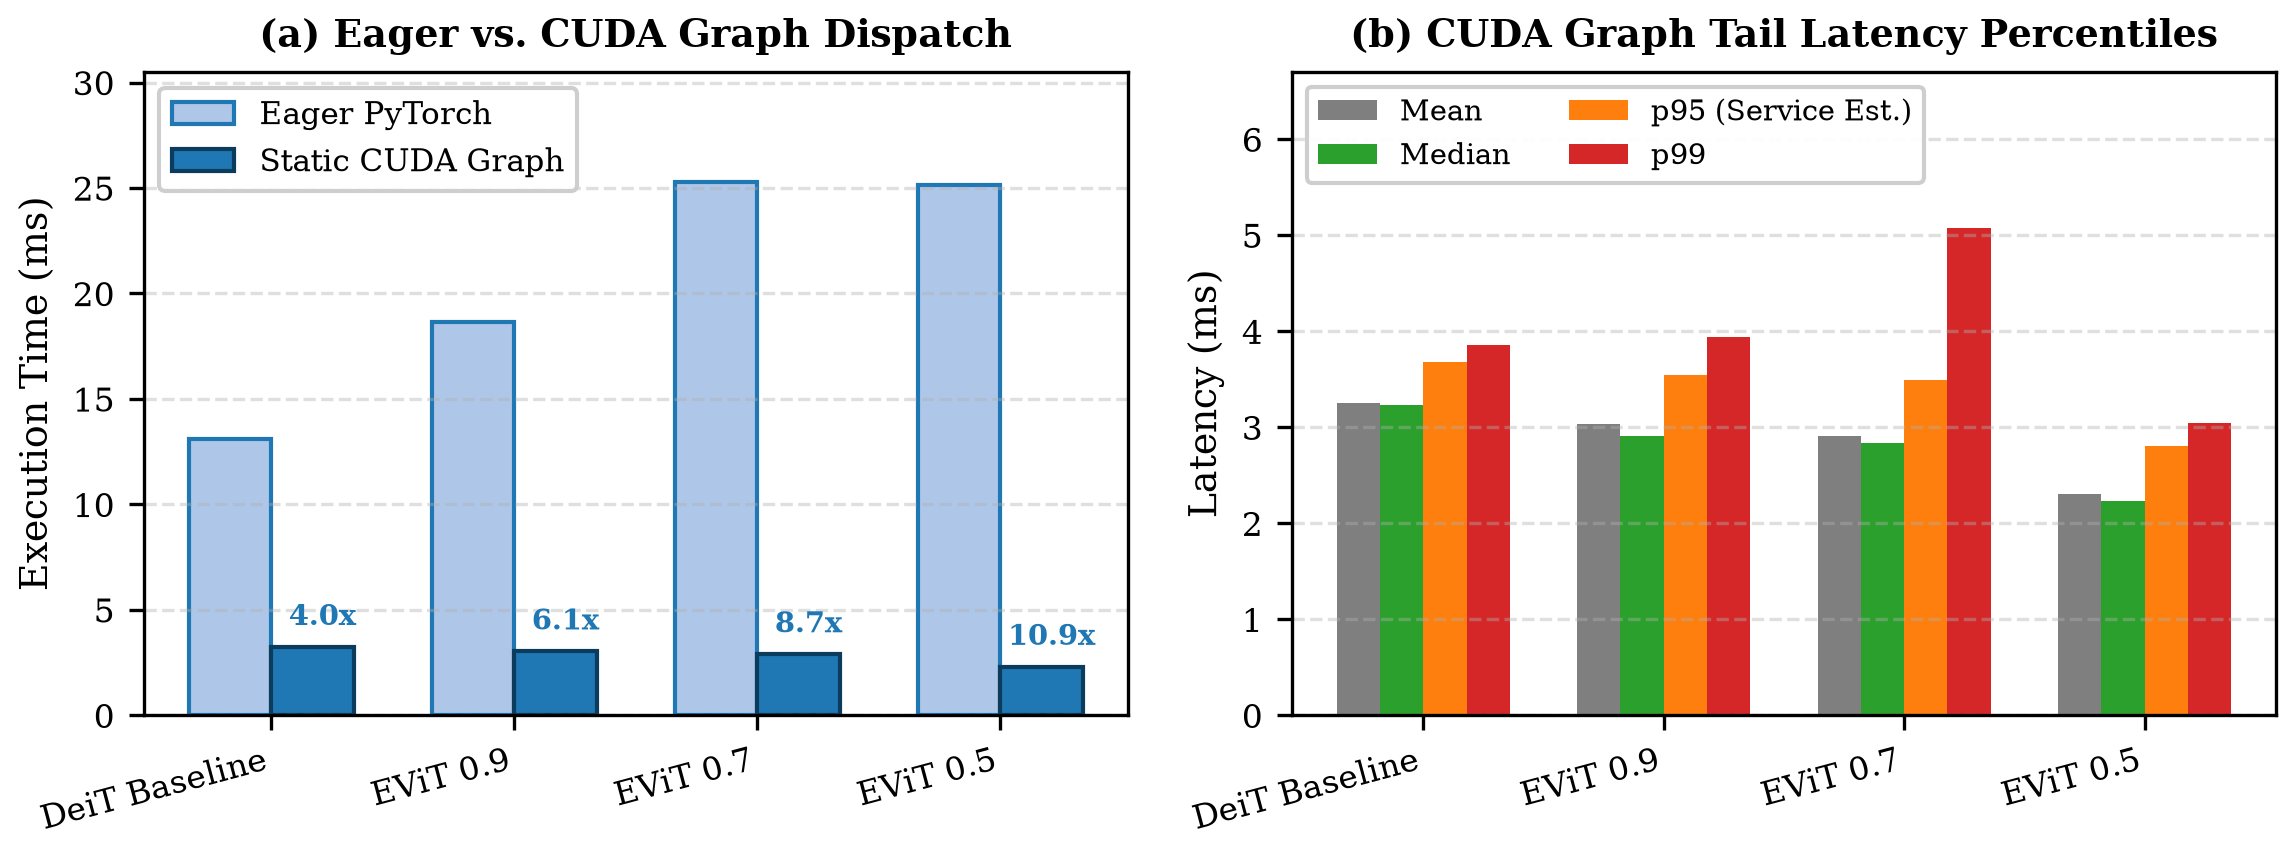
\includegraphics[width=0.88\linewidth]{figures/fig3_gpu_latency_profiles.png}
\caption{Physical GPU latency profiling on NVIDIA RTX 4060: (a) Eager PyTorch vs.\ static CUDA Graph execution, illustrating the 4.0x--10.9x speedup from kernel launch elimination; (b) Empirical tail latency percentiles (Mean, Median, p95, p99) across token pruning configurations.}
\label{fig:latency_profiles}
\end{figure*}

\subsection{Multi-Seed Validation Study}
To rigorously determine whether the observed performance improvements of K07-CB-CMPR are reproducible, we conducted a matched three-seed validation study across Seeds 42, 123, and 456. Every paired run utilized identical data splits, preprocessing transforms, loss configurations, optimizer schedules, and validation-based checkpoint selection rules.

As reported in Table~\ref{tab:multi_seed}, K07-CB-CMPR demonstrates consistent, statistically verified improvements:
\begin{enumerate}
    \item \textbf{Top-1 Accuracy Superiority:} Across all three seeds, CMPR consistently outperforms pure CB-CE ($+1.05$~pp, $+1.70$~pp, and $+1.35$~pp), yielding a mean paired improvement of $\mathbf{+1.37 \pm 0.33}$~percentage points ($77.88 \pm 0.15\%$ vs.\ $76.52 \pm 0.46\%$). An exploratory paired $t$-test confirms statistical significance at $t = 7.19, p = 0.0188$ ($p < 0.05$). We explicitly identify this test as exploratory due to the $N=3$ sample size ($df=2$).
    \item \textbf{Stabilization of Training Variance:} Teacher margin regularization dramatically stabilizes training across random initializations. The sample standard deviation of Top-1 accuracy drops from $\sigma = 0.46\%$ to $\sigma = 0.15\%$---representing a \textbf{67.4\% reduction in sample standard deviation} (and an 89.4\% reduction in variance $\sigma^2$).
    \item \textbf{Elimination of False-Positive Bleed:} Pure CB-CE penalizes majority-class confidence to boost rare classes. CMPR halts this bleed, boosting City Street recall by $\mathbf{+5.35 \pm 1.28}$~pp ($81.23\% \to 86.58\%$). In raw image counts, CMPR correctly classifies \textbf{+475 (seed 42), +745 (seed 123), and +752 (seed 456)} additional City Street frames. Weighted-F1 increases strictly across all seeds ($+0.88 \pm 0.25$~pp).
\end{enumerate}

\subsection{Mathematical Decomposition of the Gas Station Support Effect}
An essential finding of our integrity audit is the behavior of the unweighted six-class Macro-F1 metric. While Top-1 accuracy, Weighted-F1, City Street recall, and Tunnel F1 all improve strictly across all three seeds, six-class Macro-F1 exhibits a mean paired decrease of $-2.06 \pm 2.03$~pp ($+0.27$~pp on seed 42, $-3.45$~pp on seed 123, $-2.99$~pp on seed 456).

We decompose the six-class Macro-F1 delta into the direct contribution of the Gas Station class and the combined contribution of the remaining five classes:
\begin{align}
\Delta \text{Macro-F1}_{\text{6-class}} &= \underbrace{\frac{1}{6}\Delta F_{1,\text{Gas}}}_{\text{Gas Station Contrib.}} + \underbrace{\frac{1}{6} \sum_{c \neq \text{Gas}} \Delta F_{1,c}}_{\text{Remaining 5 Classes}}
\end{align}

Our mathematical audit reveals:
\begin{enumerate}
    \item \textbf{Extreme Sensitivity of $n=6$ Support:} The entire 19,902-image test split contains exactly \textbf{6 Gas Station images} (0.030\% of test set). In each seed, pure CB-CE correctly predicts exactly 2 more Gas Station images than CMPR (4 vs.\ 2 on seed 42, 4 vs.\ 2 on seed 123, 2 vs.\ 0 on seed 456). Because the denominator is 6, these 2 images shift Gas Station recall by $33.33\%$ and its F1 score by $25\%$--$30\%$. In the unweighted Macro-F1 average, this singular class imposes a direct mathematical penalty of \textbf{$-4.20$~pp to $-4.45$~pp}.
    \item \textbf{Strict Superiority Across the Remaining Five Classes:} On the remaining five classes, CMPR delivers a strictly positive net contribution in all three seeds ($+0.715\%$, $+0.752\%$, and $+1.453\%$).
    \item \textbf{Supplementary Diagnostic Metric:} When Gas Station is excluded as a supplementary sensitivity check, \textbf{Five-Class Macro-F1 is strictly superior in 100\% of seeds}, increasing by $\mathbf{+1.17 \pm 0.50}$~pp ($64.74 \pm 1.04\% \to 65.91 \pm 0.56\%$).
    \item \textbf{The Global Trade-off:} To capture those 2 additional Gas Station images, pure CB-CE misclassifies 475 to 752 City Street images. CMPR prevents this widespread error bleed, resulting in over 650 more correctly classified images overall.
\end{enumerate}

\section{Computational Efficiency and Hardware Benchmarking}

\subsection{Physical GPU Latency Profiling}
Hardware latency benchmarks were conducted on a dedicated NVIDIA GeForce RTX 4060 Laptop GPU running under Windows 11 and CUDA 12.1. Following 50 warmup iterations, execution times were captured across 200 consecutive iterations on the CUDA timeline using \texttt{torch.cuda.Event(enable\_timing=True)}, illustrated in Fig.~\ref{fig:latency_profiles}.

\begin{table}[t]
\centering
\caption{Physical GPU Profiling on NVIDIA RTX 4060 (FP32, Batch Size 1, Static CUDA Graphs)}
\label{tab:latencies}
\resizebox{\columnwidth}{!}{%
\begin{tabular}{lcccccc}
\toprule
Model Configuration & Keep ($k$) & Mean & Med. & \textbf{p95 ($C_m$)} & p99 & FPS \\
\midrule
DeiT-Small Baseline & 1.00 & 3.250~ms & 3.231~ms & \textbf{3.683~ms} & 3.859~ms & 417.1 \\
EViT K09 + CB-CMPR & 0.90 & 3.039~ms & 2.914~ms & \textbf{3.543~ms} & 3.939~ms & 469.0 \\
\textbf{EViT K07 + CB-CMPR} & \textbf{0.70} & \textbf{2.905~ms} & \textbf{2.834~ms} & \textbf{3.491~ms} & \textbf{5.080~ms} & \textbf{557.3} \\
EViT K05 + CB-CMPR & 0.50 & 2.308~ms & 2.236~ms & \textbf{2.806~ms} & 3.047~ms & 610.4 \\
\bottomrule
\end{tabular}%
}
\end{table}

\begin{table}[t]
\centering
\caption{Arithmetic Complexity, Batch Latency, and Throughput}
\label{tab:efficiency_summary}
\resizebox{\columnwidth}{!}{%
\begin{tabular}{lccccc}
\toprule
Model Configuration & GMACs & Eager BS1 Lat. & BS64 Lat. & BS64 Throughput & VRAM \\
\midrule
DeiT-Small Baseline & 4.60 & 13.04~ms (p99: 17.14) & 154.1~ms & 415.2~FPS & 350.3~MB \\
EViT K09 & 4.03 & 16.78~ms (p99: 27.52) & 134.2~ms & 476.9~FPS & 370.7~MB \\
\textbf{EViT K07} & \textbf{3.03} & \textbf{15.48~ms (p99: 19.88)} & \textbf{101.8~ms} & \textbf{629.0~FPS} & \textbf{350.6~MB} \\
EViT K05 & 2.31 & 14.57~ms (p99: 19.04) & 80.5~ms & 794.8~FPS & 350.6~MB \\
\bottomrule
\end{tabular}%
}
\end{table}

As detailed in Table~\ref{tab:latencies} and Table~\ref{tab:efficiency_summary}:
\begin{enumerate}
    \item \textbf{Eager Mode Bottleneck vs.\ CUDA Graphs:} In eager PyTorch at batch size 1, dynamic token indexing and driver dispatch cause mean latencies of 13.04~ms to 16.78~ms. Static CUDA Graphs eliminate CPU launch overheads, accelerating DeiT by \textbf{4.0x} (13.04~ms $\to$ 3.25~ms) and EViT K07 by \textbf{5.3x} (15.48~ms $\to$ 2.91~ms).
    \item \textbf{Throughput Scaling:} In multi-frame serving (batch size 64), EViT $k=0.7$ scales throughput to \textbf{629.0 FPS}---a \textbf{+51.5\% throughput speedup} over DeiT-Small (415.2 FPS), directly enabled by the 34.1\% reduction in MACs (3.03 vs.\ 4.60 GMACs).
    \item \textbf{Tail Latencies \& Non-WCET Classification:} The reported p95 and p99 values are empirical statistical percentiles from measured sample distributions and \textbf{are NOT formal deterministic Worst-Case Execution Times (WCET)}. Crucially, in eager mode at batch size 1, EViT K07 exhibits an empirical p99 latency of \textbf{19.88~ms}, which exceeds the 16.67~ms frame interval of a 60~Hz camera. This confirms that our framework operates in the \textbf{soft real-time domain}.
\end{enumerate}

\begin{figure*}[t]
\centering
\begin{minipage}{0.485\textwidth}
  \centering
  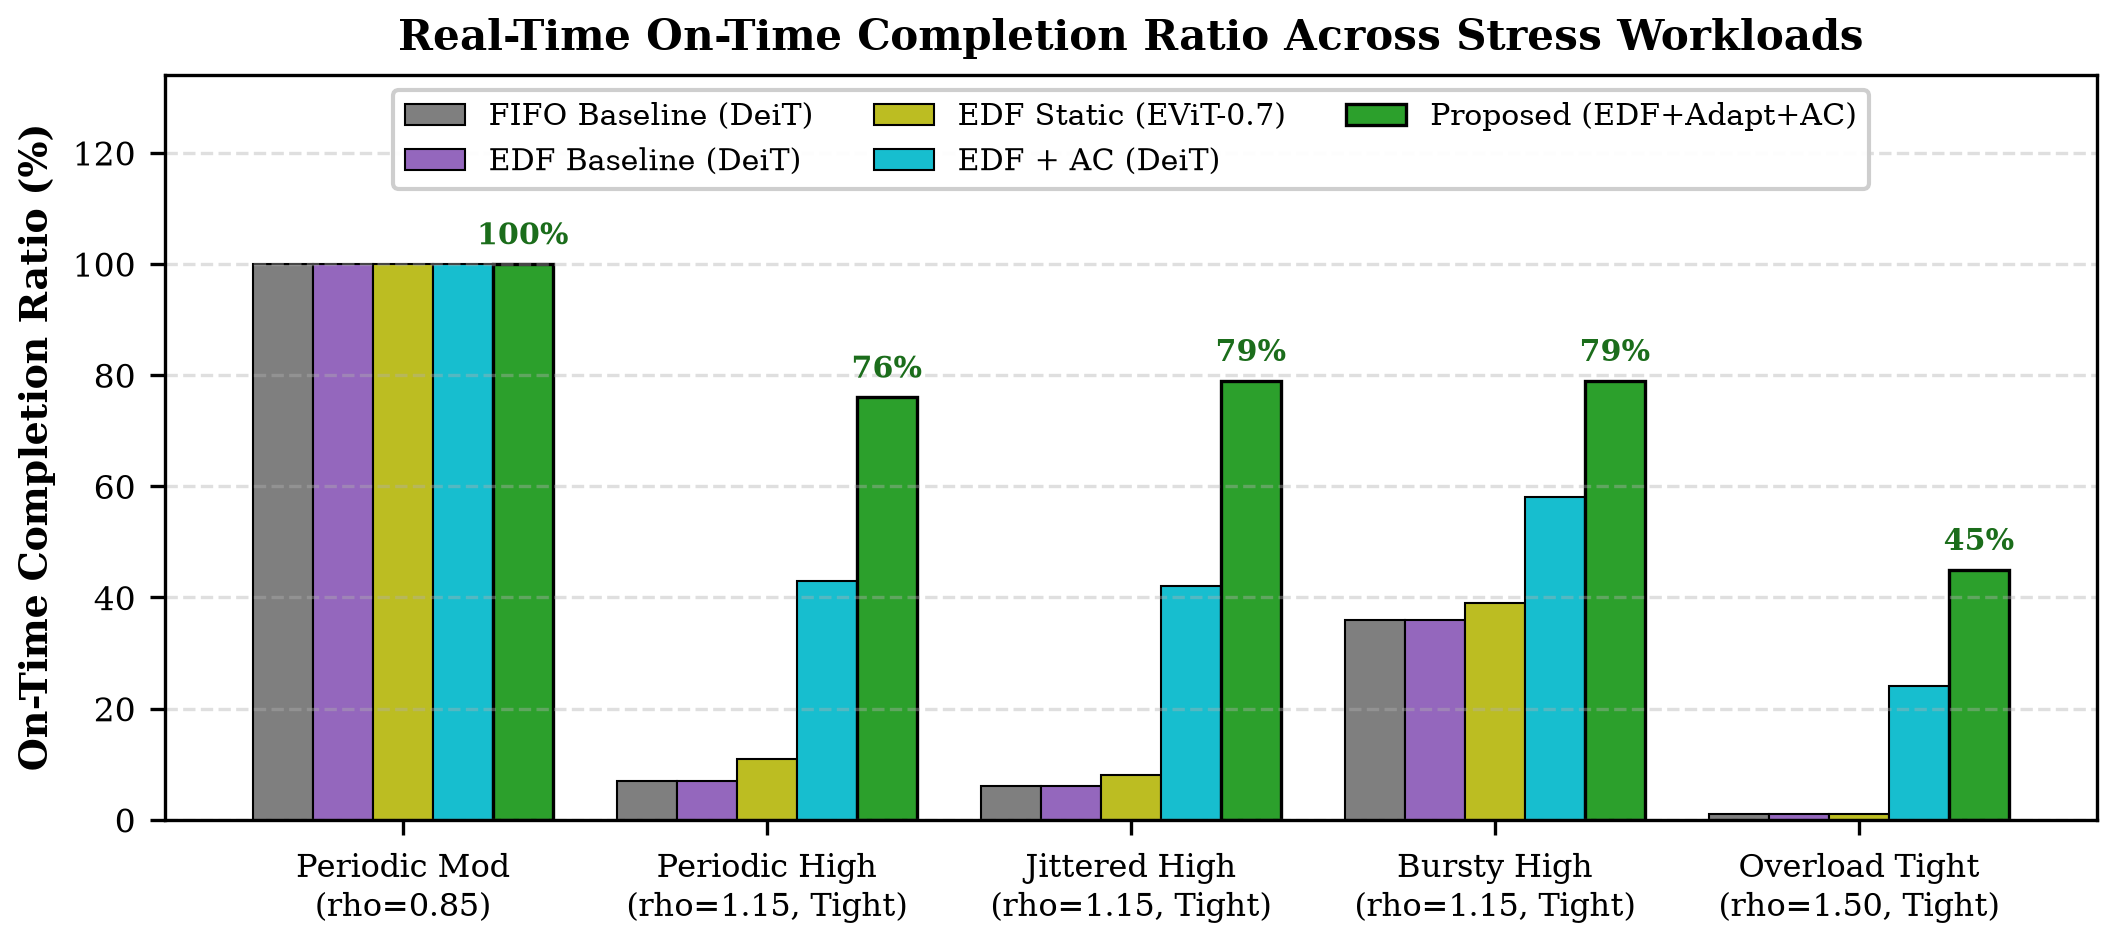
\includegraphics[width=\linewidth]{figures/fig4_scheduling_ontime_comparison.png}
  \vspace{-12pt}
  \caption{Real-time on-time completion ratio comparison across representative stress workloads for baseline and proposed policies, showing the +69~pp and +73~pp gains under heavy traffic saturation.}
  \label{fig:ontime_comparison}
\end{minipage}\hfill
\begin{minipage}{0.485\textwidth}
  \centering
  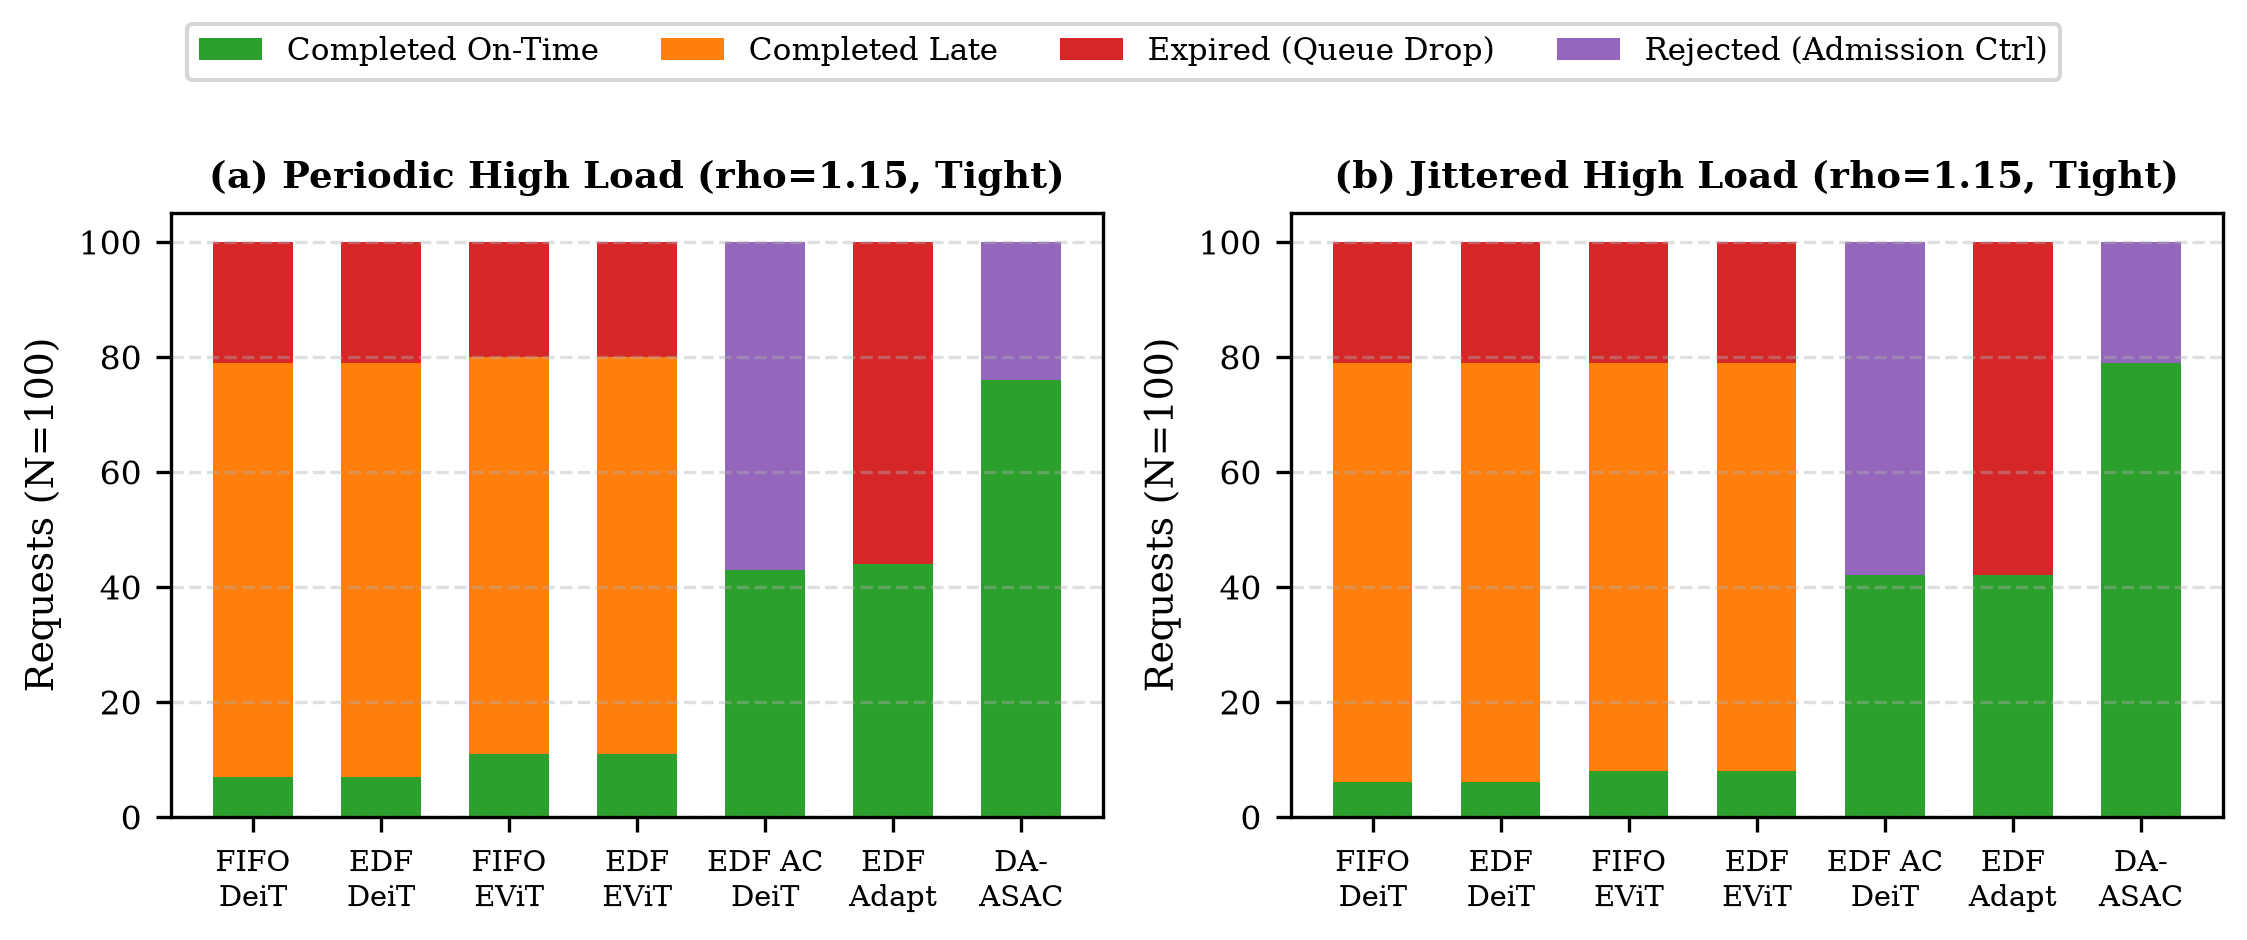
\includegraphics[width=\linewidth]{figures/fig5_request_outcomes_stacked.png}
  \vspace{-12pt}
  \caption{Request terminal outcome composition ($N=100$) under severe traffic loads: (a) Periodic high load ($\rho=1.15$, tight deadlines) and (b) Jittered high load ($\rho=1.15$, tight deadlines). Admission control filters infeasible traffic early (purple), eliminating cascading queue expirations (red) and late completions (orange) to preserve on-time completion (green).}
  \label{fig:stacked_outcomes}
\end{minipage}
\end{figure*}

\section{Scheduling and Admission Control}

\subsection{Priority Queues and Tie-Breaking}
The real-time scheduler manages pending inference requests in a binary min-heap:
\begin{itemize}
    \item \textbf{FIFO Queue:} Elements are $(A_i, \, \text{counter}, \, \text{id}_i, \, r_i)$. Ordered by arrival timestamp $A_i$. Ties are broken by monotonic request counter.
    \item \textbf{EDF Queue:} Elements are $(D_{\text{abs}, i}, \, A_i, \, \text{counter}, \, \text{id}_i, \, r_i)$. Ordered primarily by earliest absolute deadline $D_{\text{abs}, i}$, secondarily by arrival time $A_i$, and tertiarily by monotonic counter.
\end{itemize}

\subsection{Runtime Scheduling Algorithm (DA-ASAC)}
The complete dispatching and admission control logic is formalized in Algorithm~\ref{alg:da_asac}. The system operates under non-preemptive GPU semantics: once an inference graph begins execution on the GPU command processor, it runs to completion without interruption.

\begin{algorithm}[t]
\caption{Deadline-Aware Adaptive Scheduling and Admission Control (DA-ASAC)}
\label{alg:da_asac}
\begin{algorithmic}[1]\small
\REQUIRE Incoming request $r_i = (A_i, D_{\text{rel}, i}, D_{\text{abs}, i}, \mathbf{x}_i)$, Ready queue $Q$, Candidate model suite $\mathcal{M} = \{m_0, m_1, m_2, m_3\}$ sorted by descending validation accuracy, Empirical p95 service times $\{C_m\}$, GPU busy timestamp $t_{\text{busy}}$, Minimum service time $C_{\min} = C_{m_3}$.
\STATEx \textbf{// Phase 1: Queue-Tail Admission Control at Arrival}
\STATE \textbf{Procedure} \textsc{OnRequestArrival}($r_i$):
\STATE \quad $t_{\text{start}} \leftarrow \max(\text{current\_time}(), \, t_{\text{busy}})$
\STATE \quad $W_Q \leftarrow \sum_{q \in Q} C_{\text{est}}(q)$ \COMMENT{Accumulate queued workload}
\STATE \quad $t_{\text{pred\_finish}} \leftarrow t_{\text{start}} + W_Q + C_{\min}$
\IF{$t_{\text{pred\_finish}} \le D_{\text{abs}, i} + 10^{-6}$}
    \STATE $Q.\textsc{Insert}(D_{\text{abs}, i}, \, A_i, \, \text{counter}++, \, r_i)$ \COMMENT{EDF Priority Queue}
    \STATE $r_i.\text{state} \leftarrow \text{ADMITTED}$
\ELSE
    \STATE $r_i.\text{state} \leftarrow \text{REJECTED}$ \COMMENT{Shed infeasible load early}
\ENDIF
\STATEx \textbf{// Phase 2: Slack-Aware Adaptive Model Selection at Dispatch}
\STATE \textbf{Procedure} \textsc{OnGPUDispatch}($t_{\text{dispatch}}$):
\IF{$Q$ is empty}
    \STATE \textbf{return} \textsc{Idle}
\ENDIF
\STATE $r \leftarrow Q.\textsc{PopMin}()$ \COMMENT{Pop earliest absolute deadline}
\STATE $\mathcal{M}_{\text{feas}} \leftarrow \emptyset$
\FORALL{$m \in \mathcal{M}$}
    \STATE $\text{slack}(m) \leftarrow D_{\text{abs}} - (t_{\text{dispatch}} + C_m)$
    \IF{$\text{slack}(m) \ge 0$ \textbf{and} $\text{Acc}_{\text{val}}(m) \ge 45.0\%$}
        \STATE $\mathcal{M}_{\text{feas}} \leftarrow \mathcal{M}_{\text{feas}} \cup \{m\}$
    \ENDIF
\ENDFOR
\IF{$\mathcal{M}_{\text{feas}} \ne \emptyset$}
    \STATE $m^* \leftarrow \arg\max_{m \in \mathcal{M}_{\text{feas}}} \text{Acc}_{\text{val}}(m)$ \COMMENT{Break ties by larger slack}
    \STATE $t_{\text{busy}} \leftarrow t_{\text{dispatch}} + C_{m^*}$
    \STATE \textbf{Dispatch} $m^*$ on GPU via static CUDA Graph
    \STATE $r.\text{state} \leftarrow \text{COMPLETED\_ON\_TIME}$
\ELSE
    \STATE $r.\text{state} \leftarrow \text{EXPIRED}$ \COMMENT{Firm real-time drop to preserve cycles}
\ENDIF
\end{algorithmic}
\end{algorithm}

\textit{Admission Control Limitation:} The check in Phase 1 is an $O(|Q|)$ queue-tail heuristic. Under EDF scheduling, it does not re-simulate schedule reordering to guarantee that newly admitted jobs do not cause previously queued requests to miss their deadlines.

\section{Discrete-Event Simulation Results}

\subsection{Simulation Performance Across 70 Configurations}
To evaluate scheduling resilience under reproducible traffic stress, we constructed a synthetic workload suite modeling periodic, jittered, bursty, and overload traffic across four traffic intensities ($\rho \in \{0.50, 0.85, 1.15, 1.50\}$) and tight, moderate, and loose deadline constraints ($N=100$ requests per workload).

Table~\ref{tab:results} summarizes the on-time completion ratio across all ten workloads and seven scheduling policies (70 configurations), visualized comparatively in Fig.~\ref{fig:ontime_comparison}.
\begin{enumerate}
    \item \textbf{Massive On-Time Gains Under Saturation:} Under \texttt{jittered\_high\_tight}, baseline FIFO and EDF collapse to 6\% on-time completion due to cascading queue delays. Our proposed policy achieves \textbf{79\% on-time completion (+73 percentage point net gain)}.
    \item \textbf{Periodic Saturation Defense:} Under \texttt{periodic\_high\_tight} ($\rho=1.15$), static DeiT achieves only 7\% on-time completion. The proposed policy delivers \textbf{76\% on-time completion (+69~pp)}.
    \item \textbf{Bursty Workload Resilience:} In \texttt{bursty\_high\_tight}, on-time completion increases from 36\% to \textbf{79\% (+43~pp)}.
    \item \textbf{Overload Preservation:} Under severe overload (\texttt{overload\_tight\_deadline}, $\rho=1.50$), static baselines collapse to 1\%. The proposed policy maintains \textbf{45\% on-time completion} by shedding 55 infeasible requests at arrival.
\end{enumerate}

\begin{table}[t]
\centering
\caption{On-Time Completion Ratio (\%) Across All 70 Configurations ($N=100$ Offered Requests)}
\label{tab:results}
\resizebox{\columnwidth}{!}{%
\begin{tabular}{lccccccc}
\toprule
Workload Scenario & FIFO DeiT & EDF DeiT & FIFO k0.7 & EDF k0.7 & EDF AC & EDF Adapt & \textbf{Proposed} \\
\midrule
\texttt{periodic\_low\_loose} & 100\% & 100\% & 100\% & 100\% & 100\% & 100\% & \textbf{100\%} \\
\texttt{periodic\_mod\_mod} & 100\% & 100\% & 100\% & 100\% & 100\% & 100\% & \textbf{100\%} \\
\texttt{periodic\_high\_tight} & 7\% & 7\% & 11\% & 11\% & 43\% & 44\% & \textbf{76\% (+69 pp)} \\
\texttt{jittered\_mod\_mod} & 100\% & 100\% & 100\% & 100\% & 100\% & 100\% & \textbf{100\%} \\
\texttt{jittered\_high\_tight} & 6\% & 6\% & 8\% & 8\% & 42\% & 42\% & \textbf{79\% (+73 pp)} \\
\texttt{bursty\_mod\_mod} & 98\% & 98\% & 98\% & 98\% & 98\% & 98\% & \textbf{98\%} \\
\texttt{bursty\_high\_tight} & 36\% & 36\% & 39\% & 39\% & 58\% & 58\% & \textbf{79\% (+43 pp)} \\
\texttt{overload\_mod\_deadline} & 100\% & 100\% & 100\% & 100\% & 100\% & 100\% & \textbf{100\%} \\
\texttt{overload\_tight\_deadline}& 1\% & 1\% & 1\% & 1\% & 24\% & 23\% & \textbf{45\% (+44 pp)} \\
\texttt{periodic\_low\_tight} & 100\% & 100\% & 100\% & 100\% & 100\% & 100\% & \textbf{100\%} \\
\bottomrule
\end{tabular}%
}
\end{table}

\subsection{Accounting Invariant Verification}
All 70 simulation runs were independently audited against four fundamental request-conservation equations:
\begin{align}
N_{\text{offered}} &= N_{\text{on\_time}} + N_{\text{late}} + N_{\text{rejected}} + N_{\text{expired}} \\
N_{\text{completed}} &= N_{\text{on\_time}} + N_{\text{late}} \\
N_{\text{admitted}} &= N_{\text{completed}} + N_{\text{expired}} \\
N_{\text{offered}} &= N_{\text{admitted}} + N_{\text{rejected}}
\end{align}
All 70 configurations satisfy all four conservation laws with \textbf{zero accounting errors}. As illustrated in Fig.~\ref{fig:stacked_outcomes}, under high traffic saturation, admission control filters infeasible traffic at arrival, completely eliminating cascading queue expirations and late completions.

\section{Physical GPU Hardware Trace Replay Validation}

Table~\ref{tab:replay} and Fig.~\ref{fig:replay_validation} evaluate physical GPU execution across nine representative configurations using 100 unique images sampled from the held-out BDD100K test set.

\begin{figure}[t]
\centering
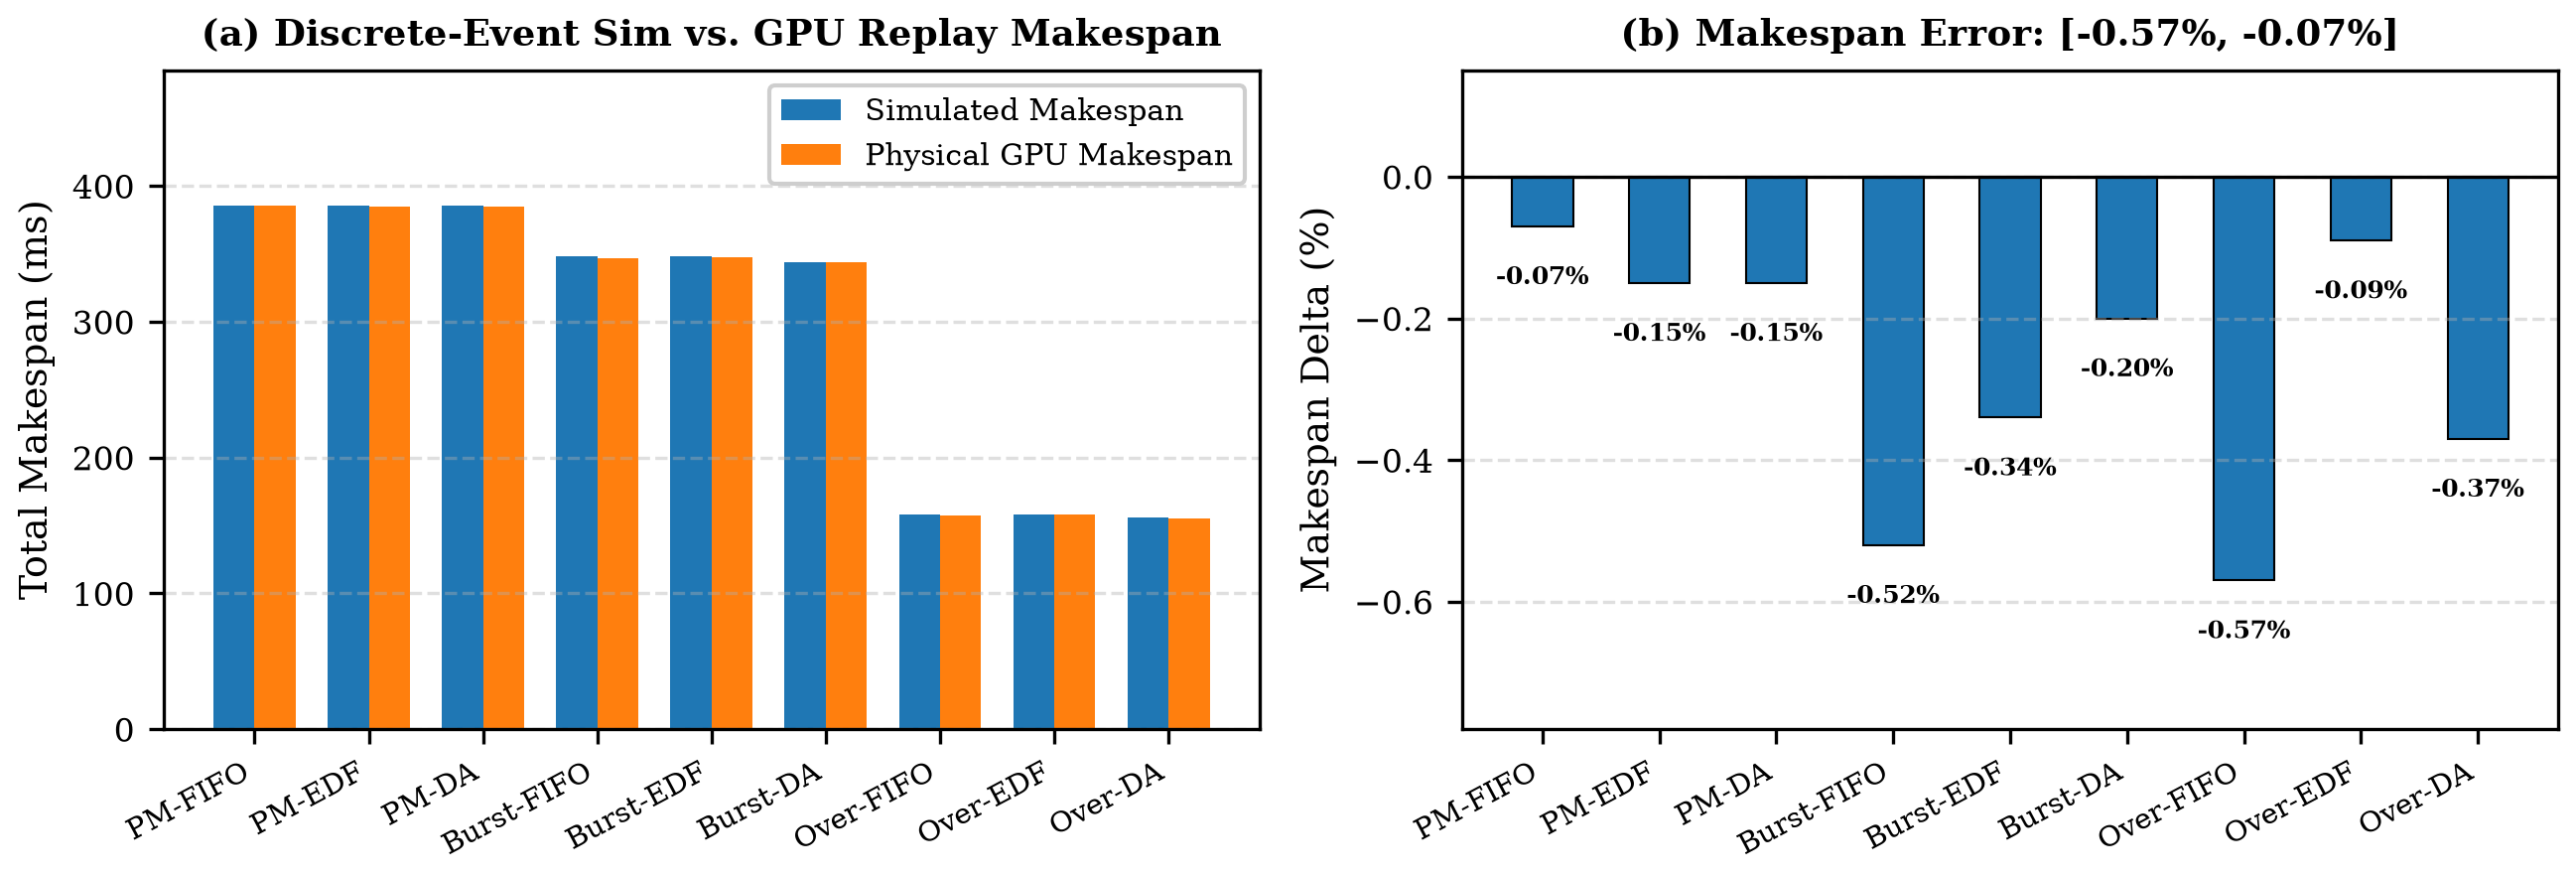
\includegraphics[width=\columnwidth]{figures/fig6_hardware_replay_validation.png}
\caption{Physical GPU hardware replay validation across 9 configurations: (a) Simulated vs.\ measured physical GPU makespan; (b) Makespan delta percentage, demonstrating tight agreement within $[-0.57\%, -0.07\%]$.}
\label{fig:replay_validation}
\end{figure}

\begin{table}[t]
\centering
\caption{Physical GPU Trace Replay vs.\ Simulation (100 Test Images)}
\label{tab:replay}
\resizebox{\columnwidth}{!}{%
\begin{tabular}{llccccc}
\toprule
Workload Scenario & Policy & Sim (ms) & GPU (ms) & \textbf{Delta} & Sim On & GPU On \\
\midrule
\texttt{periodic\_mod\_mod} & \texttt{FIFO\_DeiT} & 385.71 & 385.45 & \textbf{-0.07\%} & 100.0\% & 100.0\% \\
\texttt{periodic\_mod\_mod} & \texttt{EDF\_DeiT} & 385.71 & 385.11 & \textbf{-0.15\%} & 100.0\% & 100.0\% \\
\texttt{periodic\_mod\_mod} & \texttt{EDF\_Adap\_AC} & 385.71 & 385.12 & \textbf{-0.15\%} & 100.0\% & 100.0\% \\
\texttt{bursty\_high\_tight} & \texttt{FIFO\_DeiT} & 348.59 & 346.78 & \textbf{-0.52\%} & 36.0\% & 63.0\% \\
\texttt{bursty\_high\_tight} & \texttt{EDF\_DeiT} & 348.59 & 347.41 & \textbf{-0.34\%} & 36.0\% & 59.0\% \\
\texttt{bursty\_high\_tight} & \texttt{EDF\_Adap\_AC} & 344.19 & 343.50 & \textbf{-0.20\%} & 79.0\% & 84.0\% \\
\texttt{overload\_tight} & \texttt{FIFO\_DeiT} & 158.37 & 157.46 & \textbf{-0.57\%} & 1.0\% & 2.0\% \\
\texttt{overload\_tight} & \texttt{EDF\_DeiT} & 158.37 & 158.23 & \textbf{-0.09\%} & 1.0\% & 1.0\% \\
\texttt{overload\_tight} & \texttt{EDF\_Adap\_AC} & 155.58 & 155.00 & \textbf{-0.37\%} & 45.0\% & 60.0\% \\
\bottomrule
\end{tabular}%
}
\end{table}

\begin{enumerate}
    \item \textbf{Makespan Fidelity:} Across all nine configurations, simulation makespan matches physical GPU execution within \textbf{$-0.57\%$ to $-0.07\%$}.
    \item \textbf{Conservative Simulation Bounds:} Live GPU on-time completion ratios are systematically higher than simulated estimates (84\% vs.\ 79\% for bursty; 60\% vs.\ 45\% for overload). This divergence occurs because the simulator models per-job execution cost using the empirical 95th percentile ($C_{\text{est}} = p95$), whereas physical GPU execution times follow a distribution centered around the lower median (2.24--3.23~ms).
\end{enumerate}

\section{Discussion and Limitations}

\subsection{Synergy Between Model Adaptation and Admission Control}
Our findings demonstrate that \textbf{token pruning alone cannot solve real-time queue saturation}. In \texttt{periodic\_high\_tight}, switching statically from DeiT to EViT K07 improves on-time ratio from 7\% to only 11\%. Because the traffic arrival interval ($\Delta = 2.85$~ms) is shorter than the execution time of EViT K07 ($C_m = 3.49$~ms), queues inevitably overflow. High on-time completion requires coupling model pruning with admission control, which sheds 21\%--24\% of infeasible requests at arrival, enabling the remaining traffic to finish on time.

\subsection{Threats to Validity and Practical Limitations}
To maintain rigorous scientific standards, we highlight key limitations:
\begin{enumerate}
    \item \textbf{Soft Real-Time Scope vs.\ Formal WCET:} The reported p95 and p99 execution latencies are empirical statistical percentiles from measured sample distributions, \textbf{not formal deterministic Worst-Case Execution Times (WCET)}. The system provides soft real-time Quality-of-Service rather than hard real-time safety guarantees.
    \item \textbf{Tail Latency Frame Interval Limits:} In eager PyTorch at batch size 1, EViT K07 exhibits an empirical p99 latency of \textbf{19.88~ms}, which exceeds the 16.67~ms interval required for 60~Hz camera feeds. While static CUDA Graphs reduce median latency to 2.83~ms, the system does not certify hard 60~FPS guarantees without dedicated hardware isolation.
    \item \textbf{Synthetic Workload Traces:} Arrival patterns and deadlines are synthetic mathematical models designed to evaluate queueing stress; they do not capture physical PCIe camera bus contention or OS interrupt latency.
    \item \textbf{Sampled Replay Scope:} Live GPU hardware replay evaluated 100 canonical test images across nine configurations; the full 19,902 test set was evaluated offline.
    \item \textbf{Heuristic Admission Control:} The $O(|Q|)$ queue-tail feasibility test is an approximation and does not perform exact global EDF schedulability analysis.
    \item \textbf{Multi-Seed Sample Size:} Multi-seed validation was conducted over three independent seeds ($N=3$). While paired Top-1 improvements are statistically significant under a paired $t$-test ($p = 0.0188$), asymptotic normality assumptions are best strengthened by future five-seed expansions.
\end{enumerate}

\section{Conclusion}
We presented a deadline-aware adaptive vision transformer inference framework for soft real-time edge workloads. By co-designing EViT token pruning with smooth Class-Balanced Cross-Entropy and teacher-guided Class-Margin-Preserving Regularization (CMPR), our approach achieves $77.88 \pm 0.15\%$ Top-1 accuracy ($+1.37 \pm 0.33$~pp gain, $p = 0.0188$) on the imbalanced BDD100K driving benchmark while cutting arithmetic complexity by 34.1\% (3.03 GMACs) and boosting throughput by $+51.5\%$. When orchestrated by an earliest-deadline-first scheduler with queue-tail admission control under static CUDA Graph execution, the framework improves real-time deadline satisfaction by up to $+73$ percentage points under severe load, with physical GPU execution corroborating simulated makespans within $-0.57\%$ to $-0.07\%$.

\IEEEtriggeratref{9}
\bibliographystyle{IEEEtran}
\bibliography{references}

\end{document}
